\chapter{Image Processing Techniques}
\label{ch:imageprocessing}

\begin{figure}[htbp]
    \centering
    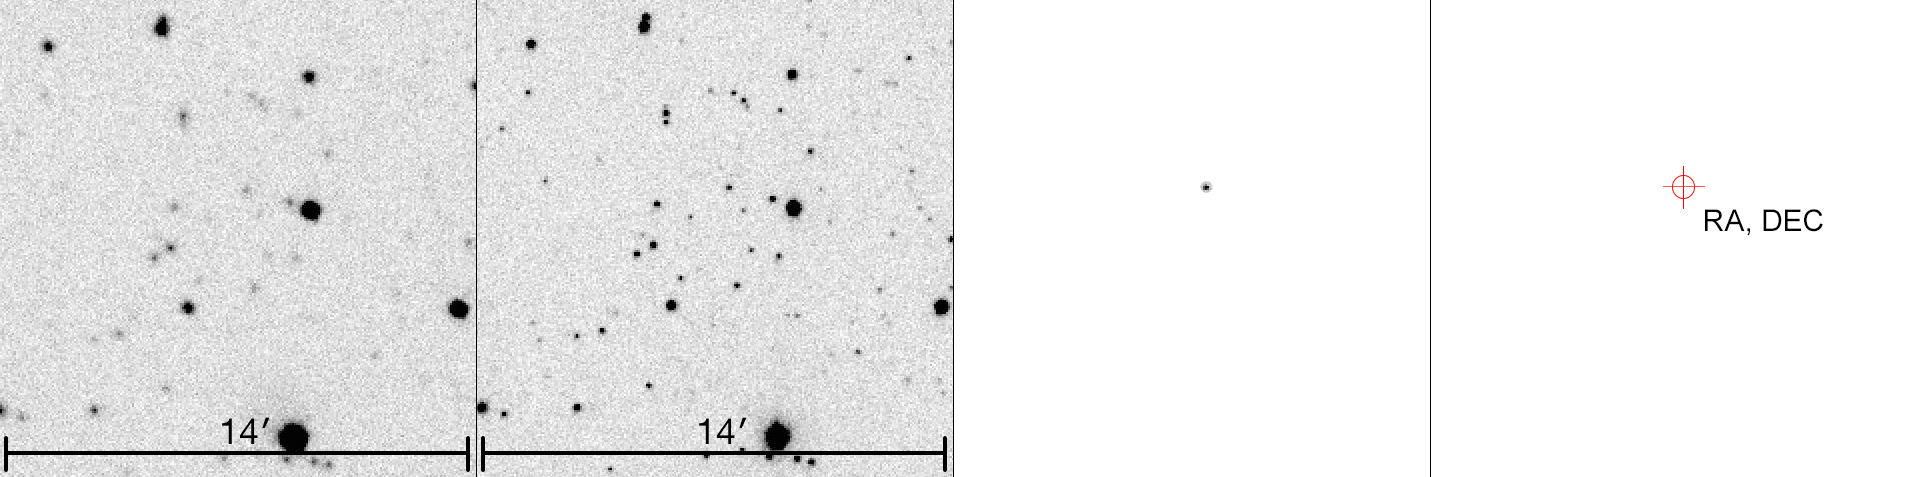
\includegraphics[width=1.0\textwidth]{images/processing.png}
    \caption{Overview of the process of image processing (images from \cite{ATLASBlog}). Note that these images were not obtained using the mentioned methods, but merely serve as illustration.}
    \label{fig:processingprocess}
\end{figure}

After capturing the image, the process of image processing can begin. This process transforms the data from the sensors to measurements needed for determining the trajectory of the asteroid. This process consists of various steps, of which an overview is provided in \autoref{fig:processingprocess}. Firstly, the image is taken by the camera. Then, various steps are undertaken to improve the quality of the image. Next, the background of the image is removed, leaving only the PSF of the target. Lastly, the center of the target is determined. As the first step consists of only a well-described calibration procedure known as \textit{flat-fielding} (e.g \cite{SMAD}, \cite{OpNav}), it will not be discussed in further detail. Therefore in this chapter only the background removal and centerfinding procedures are detailed. In addition, for completeness, some applications of neural networks for image processing will be discussed.

\section{Background Removal}
After compensating for known effects such as the fixed pattern noise described in \autoref{sec:opticalnoise}, the system obtains an image consisting of three components: The background, the noise and the \textit{transients}, such as asteroids. Thus, the signal in each pixel can be described as a linear combination of signal, background and other noise. The static background signal $B_e$ comprises primarily background stars and zodiacal light. This background signal can be removed in several ways. The most basic way is to find the value of the background light and subtract this from all signals, such as described by \cite{sextractor}. Various methods for estimating the background value of an image exist, but most methods operate under the assumption that there is always more sky than objects in the image. Therefore, if one is to plot a histogram of pixel values, the mode of this histogram will provide a reasonable assumption for the background signal.\\

There is, however, a more accurate method available at the cost of more work to remove the background objects: Because of the extremely far distance to other stars, they are essentially unmoving as seen from the space system. Consider a spacecraft in an orbit with a semi-major axis of 1 AU, with an angular resolution of 2 arcseconds per pixel (from the values in \autoref{tab:typicalcamera}). It follows from basic trigonometry that a target further away than 3.26 lightyears would provide less parallax error than the resolution of the sensor.\footnote{A more convenient unit here would be the \textit{parsec}, $1pc \approx 3.26ly$. The parsec is the distance of an object where 1 AU subtends an angle of 1 arcsecond} Of course, this is a shorter distance than even the distance to the nearest other star, Proxima Centauri at more than 4 light years. Therefore, the background can be assumed constant. Thus, it is possible to perform a procedure known as "image differencing", where a reference image is subtracted from the new image, effectively removing the background signal. Thus, the system is left with a combination of signal and the remaining noise components. The reference images can be composed of other images taken by the system itself (e.g. \cite{subtraction}), or the images can be created (e.g. \cite{PalomarPipeline}). This is possible as almost all objects responsible for the background signal are known. These objects are logged in databases such as ESA's GAIA (\cite{GAIA}), which contains positions of over one billion stars. This can be combined with ephemerides from known solar system objects, and thus the difference can be found. Then, through statistical methods targets with a large enough SNR can be found, as is shown in \autoref{fig:transientsfound}. This method will of course find more transients than just asteroids; also other phenomena such as, but not limited to, supernovae, variable stars, eclipsing binaries and new quasars will be detected. How to determine the difference between these objects is beyond the scope of this review, although some examples will be given in the final section of this chapter.

\begin{figure}[htbp]
    \centering
    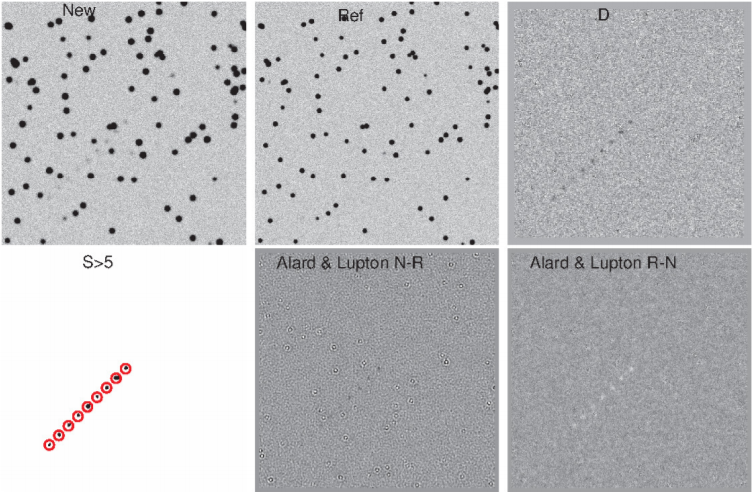
\includegraphics[width=0.8\textwidth]{images/transients.png}
    \caption{Demonstration of the image subtraction process from a series of stacked images. The path of the transient is shown in red (\cite{processingclassic}).}
    \label{fig:transientsfound}
\end{figure}

\section{Centerfinding}
With the image taken by the camera reduced to a projection of the PSF, the question remains on how to transform this imaged PSF into an angular measurement as accurately as possible. Note that it will only be possible to determine the angular position of the asteroid accurately, not its actual position, as the point spread function is not dependent on the distance to the target, and the target is too small to resolve into multiple pixels. The angular measurements will be combined with knowledge on astrodynamics in the next chapter to solve for the position of the target. However first, this angular position needs to be determined as accurately as possible. \cite{OpNav} provides an overview of the main algorithms suitable for this purpose:\\

The most simple to implement algorithm is to model a point spread function (resulting in an array $\mathbf{P}$ and calculate the correlation across the pixel grid $\mathbf{D}$ which contains the point spread function. Therefore, the challenge is to find $\mathbf{P}$ in $\mathbf{D}$. Let $\mathbf{P'}$ and $\mathbf{D'}$ be zero-mean and unit standard deviation normalized versions of the aforementioned arrays. Then, \cite{OpNav} defined the \textit{correlation array} $\rho(\Delta s, \Delta l)$ as the sum of the products of the arrays, with $\mathbf{P'}$ shifted by integer amounts $\Delta s$ and $\Delta l$ (in such as way that $\mathbf{P}$ is entirely inside the coordinates of $\mathbf{D}$:
\begin{equation}
    \rho(\Delta s, \Delta l) = \Sigma_i \Sigma_j \mathbf{P'}_{i,j} \mathbf{D'}_{i+\Delta s, j+\Delta l}
\end{equation}
In practice, this is more convenient by first computing with the unnormalized arrays:
\begin{align}
    m_d &= \Sigma \mathbf{D}_{i+\Delta s, j+\Delta l} \\
    s_d &= \Sigma \mathbf{D}^2_{i + \Delta s, j+\Delta l} \\
    m_p &= \Sigma \mathbf{P}_{i,j} \\
    s_d &= \Sigma \mathbf{P}^2_{i, j} \\
    r &= \Sigma \mathbf{D}_{i+\Delta s, j+\Delta l} \mathbf{P}_{i,j}
\end{align}
Then, with $N$ the number of pixels in the summation:
\begin{equation}
    \rho(\Delta s, \Delta l) = \frac{Nr - m_d m_p}{\sqrt{\left(Ns_d - m_d^2\right)\left(Ns_p - m_p^2\right)}}
\end{equation}
This will result in a value of $\rho$ between -1 for perfect anticorrelation, and +1 for perfect correlation. Therefore, the best estimate of $\Delta s, \Delta l$ is given by the maximum of $\rho$, which can be determined to sub-pixel accuracy by e.g. interpolation. For example, consider a parabola fitted to the following points:
\begin{align}
    \rho_0 &= \rho(\Delta s, \Delta l) \\
    \rho_- &= \rho(\Delta s-1, \Delta l) \\
    \rho_+ &= \rho(\Delta s+1, \Delta l)
\end{align}
It follows that the maximum value of $\rho$ is found at:
\begin{equation}
    x = 2\frac{\rho_+ + \rho_- - 2\rho_0}{\rho_+ - \rho_-}
\end{equation}
Similarly, the second coordinate can be solved for $y$. Note that the approach of finding the correlation requires some imprecise interpolation. This might be unwanted, as \cite{veryshortarcs} results indicate a large drop in performance for measurements with a precision worse than 4 or 5 decimals (in degrees). Therefore, a slightly more complicated process which does not require interpolation is to fit some analytical function to the data. \cite{OpNav} mentions that the choice of which function to use is not very important, as long as it is reasonable. Some possibilities include the Lorentzian function (\cite{lorentzian}):
\begin{equation}
    B(s, l) = \frac{h}{1+(r / r_0)^2} + B_e
\end{equation}
Or the two-dimensional Gaussian (\cite{OpNav}):
\begin{align}
    B(s,l) &= \frac{h}{2\pi} \mathrm{exp}\left(-\frac{(s-s_c)^2 + (l-l_c)^2}{s\sigma^2}\right) + B_e \\
    &\equiv h \mathcal{N}\left(\frac{s-s_c}{\sigma}\right) \mathcal{N}\left(\frac{l-l_c}{\sigma}\right) + B_e \\
    &\equiv h \mathcal{N}(\xi(s))\mathcal{N}(\eta(l)) + B_e
\end{align}
With $\sigma$ the standard deviation in the pixels, $h$ the magnitude of the pixel values in $DN$ and $B_e$ the background signal. Where $\mathcal{N}(z)$ is the zero-mean normal distribution with $z$ standard deviation. The functions $\xi(s)$ and $\eta(l)$ are normalisation functions to zero mean and unit variance. As this constitutes a density function, it follows that the values of the pixels should be the integral over the area of the pixel. Note that, since background removal is performed prior, it is assumed that $B_e = 0$:
\begin{align}
    DN(s,l) &= \int_{s-0.5}^{s+0.5} \int_{l-0.5}^{l+0.5} B(x,y)dy dx \\
    &= h\left[erf(\xi(s+0.5)) - erf(\xi(s-0.5))\right]\left[erf(\eta(l+0.5))-erf(\eta(l-0.5))\right]
\end{align}
With $erf(z)$ the Gaussian error function:
\begin{equation}
    erf(z) = \frac{2}{\sqrt{\pi}}\int_0^ze^{-t^2}dt
\end{equation}
The function fitting concerns the variables $s_c, l_c, h, \sigma$. These begin by estimation from the data, from which the expected $DN$ values can then be computed. Subtraction from the measured values yield an array of residuals, which can be used to iteratively converge to a solution through e.g. gradient descent, or by computing the first-order partial derivatives of $DN(s,l)$ with respect to $s_c, l_c,h, \sigma$ and performing a non-linear least-squares fit. \\

After performing one of these estimations, \autoref{eq:cameraprojection} can be used to determine the unit vector to the target in relation to the optical axis of the camera. If the unit vector of the optical axis is known, a solution in e.g. celestial coordinates follows trivially. Note that the vector of the optical axis can be determined very precisely, as the camera can also function as a star tracker, such as demonstrated by the NEOSSat mission exhibited in \autoref{ssec:NEOSSat}.

\section{Applications of Neural Networks}

Like any field of technical research, astronomy is faced with the challenge and opportunity of exponentially increasing amount of data to process. For this reason, big data techniques such as machine learning and especially artificial neural networks have become widely researched. A further discussion of the workings of artificial neural networks and how to use them for the proposed research is given in \autoref{sec:ANN}. In this section, only an overview of the current research regarding neural networks in astronomical image processing is given. It is assumed the reader has a basic familiarity with convolutional neural networks; else they are advised to refer to some of the excellent literature on this topic such as \cite{nnbooktwo} or \cite{nnbookfour}\footnote{An online version of this book is available for free at \url{https://www.deeplearningbook.org/}.}.\\

Convolutional Neural Networks (CNN's) are the subject of several ongoing research projects. A few interesting results are presented here to give an overview of the current state of research. The first application of CNN's is in the determination of whether or not something is truly a target, or merely noise or an image artifact. CNN's provide an effective way of discriminating between these without human intervention.\\

\begin{figure}[htbp]
    \centering
    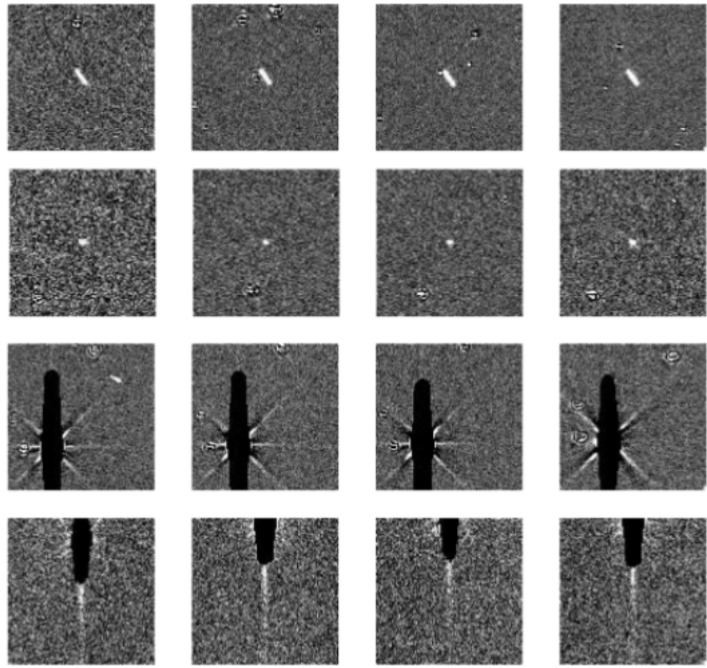
\includegraphics[width=0.5\textwidth]{images/atlascnn.png}
    \caption{Some images from ATLAS data. The first two rows show actual detections of asteroids, whereas the latter two rows show visual artifacts. Note how the white streaks in the bottom images might be mistakes for astroid tracks in a more simple algorithm (\cite{AtlasDL}.)}
    \label{fig:AtlasCNN}
\end{figure}

Firstly, \cite{AtlasDL} examine the possibility of using a two stage deep learning classifier on data gathered by the ATLAS (\autoref{ssec:ATLAS}) telescopes. In \autoref{fig:AtlasCNN}, an example is given on the types of images the classifier must process. The system is capable of classifying eight different classes: bright comets, asteroid streaks, cosmic rays, and "other astronomical objects", as well as several types of noise and visual artifacts. The network is trained entirely using real-world data. Using a CNN for feature extraction coupled with a dense classifier allows the authors to obtain a 0.4\% false negative rate coupled with a 9.1\% false positive rate. In practice, this means a reduction of over 90\% in workload for humans who would otherwise have to classify the images. \\

\begin{figure}[htbp]
    \centering
    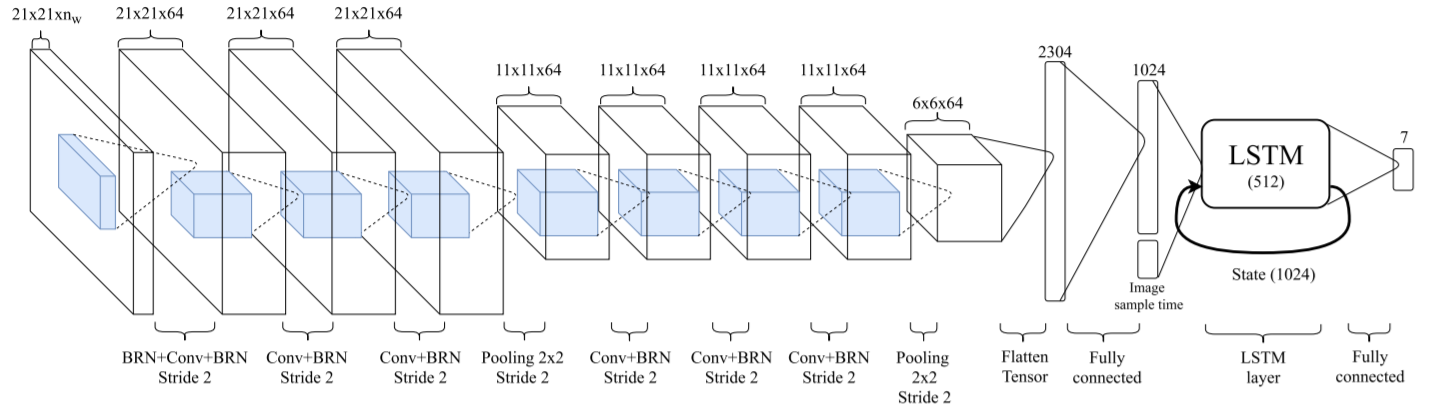
\includegraphics[width=1.0\textwidth]{images/ztfclassifier.png}
    \caption{Schematic of the network used by \cite{processingDLtwo} for classification into seven classes of observations.}
    \label{fig:ztfnetwork}
\end{figure}

\begin{figure}[htbp]
    \centering
    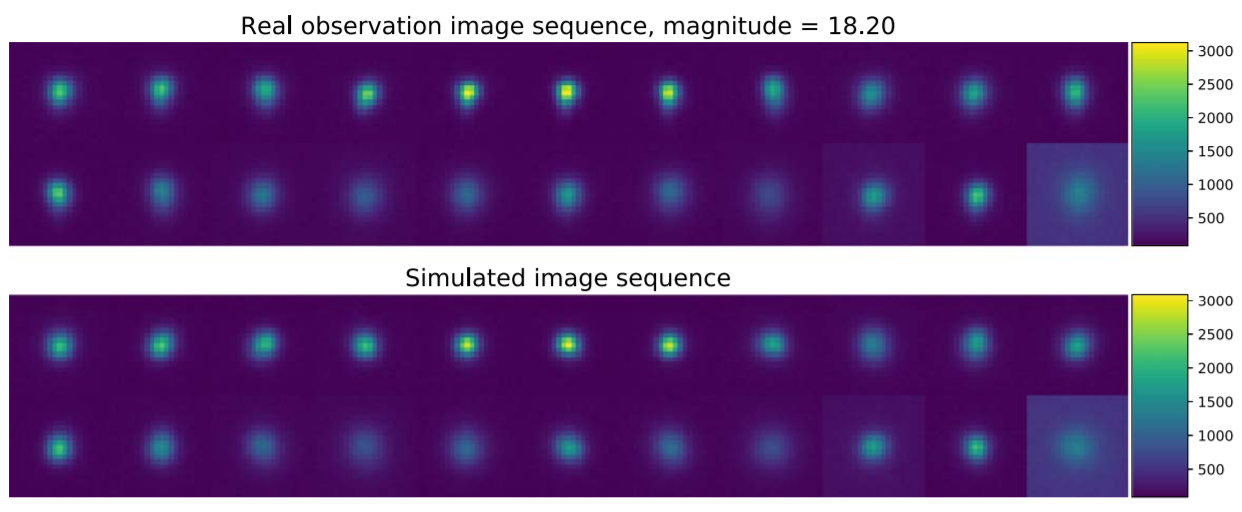
\includegraphics[width=0.7\textwidth]{images/ztfsimulation.png}
    \caption{Comparison of real and simulated image sequences from \cite{processingDLtwo}.}
    \label{fig:ztfsim}
\end{figure}

Next to ATLAS, the Zwicky Transient Facility (\autoref{ssec:palomar}) is used as a testbed for several processing algorithms to be used on the Large Synoptic Survey Telescope. \cite{supernovacnn} provided the groundwork for application of CNN's at the Zwicky Transient Facility in detecting supernovae, and \cite{processingDLone} expanded greatly on this research. The authors use a deep convolutional neural network to classify images as target or bogus, achieving over 99\% accuracy, precision and recall, and outperforming previously used random forest (a type of machine learning) classifiers. The network is also trained entirely on real data. An example of using simulated data to effectively train the network was given by \cite{processingDLtwo}: without performing image subtraction, the authors use a convolutional neural network for feature extraction followed by LSTM recurring neural network. An schematic of the network architecture is shown in \autoref{fig:ztfnetwork}. They manage to obtain results similar to classical processing methods without performing the compultationally intensive steps associated with those methods. Perhaps more interesting, is that the network was trained on a completely simulated dataset, and later validated on data captured by the telescopes. \autoref{fig:ztfsim} provides an example of a simulated data sequence compared to a real data sequence. \\

\begin{figure}[htbp]
    \centering
    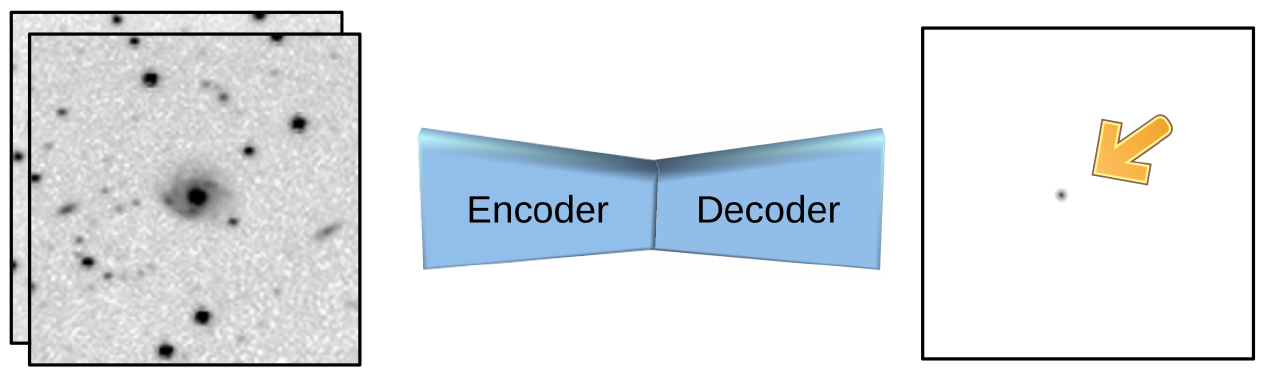
\includegraphics[width=0.9\textwidth]{images/encdec.png}
    \caption{The system trained by \cite{autoencoder} and its results.}
    \label{fig:autoencoder}
\end{figure}

As a last impressive example of the power of CNN's in image processing, \cite{autoencoder} present another system to be tested at the Zwicky Transient Facility. The author make use of an autoencoder: a type of neural network architecture where the network is trained to replicate its input as accurately as possible. The ingenuity in the autoencoder resides in enforcing a dimensionality reduction on the data (by creating a "bottleneck" in the network), thus forcing the network to learn a more compact representation of the data. It is thus hoped that all patterns in the data are learned and preserved, and any noise will not be encoded and "lost" in the deconding process. \cite{autoencoder} take a small sidestep from this concept, instead providing the 16-layer fully convolutional autoencoder with both an image taken by the telescope, containing a target and a reference image, as discussed earlier. They then train the system to reproduce the image of just the target. Thus, a method of processing the image into purely the PSF of the target is obtained without the need for any classification or image subtraction. The system is trained on a combination of real data and augmented data from freely available datasets. An example of the system is shown in \autoref{fig:autoencoder}, which demonstrates its powerful processing. The authors demonstrate decent performance ($\approx$80\% recall) for relative magnitudes of around -0.1 of the transient compared to the background, and very good (close to 100\%) for relative magnitudes of -0.15 and beyond. The system yields vastly cleaner images of the PSF than e.g. \cite{processingclassic}, although the authors admit not being experts in the application of the latter. \\

In conclusion, neural networks open some very exiting possibilities for processing this kind of data, and can be applied using both real and simulated data. Challenges lie in verifying and validating the data, as well as some common pitfalls encountered in the training of neural networks, which will be discussed in more detail in the next chapter.